\documentclass[pdflatex,sn-mathphys-num]{sn-jnl}% Math and Physical Sciences Numbered Reference Style

\usepackage{graphicx}%
\usepackage{multirow}%
\usepackage{amsmath,amssymb,amsfonts}%
\usepackage{amsthm}%
\usepackage[title]{appendix}%
\usepackage{xcolor}%
\usepackage{textcomp}%
\usepackage{manyfoot}%
\usepackage{booktabs}%
\usepackage{algorithm}%
\usepackage{algorithmicx}%
\usepackage{algpseudocode}%
\usepackage{listings}%

\providecommand{\code}[1]{\texttt{#1}}%
\algrenewcommand\algorithmicrequire{\textbf{Input:}}
\algrenewcommand\algorithmicensure{\textbf{Output:}}

\theoremstyle{thmstyleone}%
\newtheorem{theorem}{Theorem}%
\newtheorem{proposition}[theorem]{Proposition}%

\theoremstyle{thmstyletwo}%
\newtheorem{example}{Example}%
\newtheorem{remark}{Remark}%

\theoremstyle{thmstylethree}%
\newtheorem{definition}{Definition}%

\raggedbottom

\begin{document}
\graphicspath{{figures/}}

\title[Adaptive Identification and Tracking]{Adaptive Candidate Routing for Distributed Occupant Recognition Across Multiple Building IoT-enabled Smart Spaces}

\author*[1,2]{\fnm{First} \sur{Author}}\email{iauthor@gmail.com}

\author[2,3]{\fnm{Second} \sur{Author}}\email{iiauthor@gmail.com}
\equalcont{These authors contributed equally to this work.}

\author[1,2]{\fnm{Third} \sur{Author}}\email{iiiauthor@gmail.com}
\equalcont{These authors contributed equally to this work.}

\affil*[1]{\orgdiv{Department}, \orgname{Organization}, \orgaddress{\street{Street}, \city{City}, \postcode{100190}, \state{State}, \country{Country}}}

\affil[2]{\orgdiv{Department}, \orgname{Organization}, \orgaddress{\street{Street}, \city{City}, \postcode{10587}, \state{State}, \country{Country}}}

\affil[3]{\orgdiv{Department}, \orgname{Organization}, \orgaddress{\street{Street}, \city{City}, \postcode{610101}, \state{State}, \country{Country}}}


\abstract{This work proposes a privacy-aware biometric-embedding routing mechanism for occupant identification and tracking across multiple buildings in IoT-enabled smart spaces. Centralized galleries raise privacy concerns, while distributed galleries incur overhead in locating the appropriate building before recognition. The proposed approach models the environment using a Distributed State Transition System (DSTS), where states represent occupant presence probabilities, events represent biometric recognition, and transitions describe state evolution. Each building shares a Bloom filter constructed from locality-sensitive hashing (LSH) codes of its registered occupants. A captured face generates $L$ codes, which are checked against all filters to rank candidate buildings. Only the highest-ranked buildings verify the face against their reference embeddings. Experiments involving 500 CASIA-WebFace identities across 10 buildings, averaged over 20 random assignments, achieve 92.81\% recognition accuracy, compared with 95.50\% for centralized recognition. An adaptive strategy querying additional buildings when rankings are ambiguous achieves 92.95\% accuracy while contacting an average of 2.54 buildings per query. The mean face and acceptance angle are derived from reference images, whereas $K$ and $P$ were selected using test accuracy; alternative configurations are therefore reported. The filter false-positive rate is 3.54\%, exceeding the configured 1\% because of LSH code collisions. As buildings increase from 10 to 100, the proportion of queries whose true building appears in the shortlist decreases from 94.8\% to 87.0\%. Filter access enables building-membership inference with an AUC of 0.93. Computational costs are estimated rather than measured, and encryption and unknown visitors remain unevaluated.}
\keywords{Occupant identification and tracking, Distributed state transition system, Smart spaces, Locality-sensitive hashing, Bloom filter, Face recognition}


\maketitle


\section{Introduction}

Camera networks are widely deployed across IoT-enabled smart spaces to monitor occupants and support occupant-specific building-level services~\cite{SM2022,hou2017}. These applications require reliable occupant identification and tracking to associate facial observations with the correct individuals. When such services span multiple buildings, identity resolution depends on how biometric reference data are maintained and accessed across the buildings. Centralized architectures maintain a common database of reference face embeddings, whereas distributed architectures retain biometric reference data within individual buildings. Centralized approaches concentrate sensitive biometric data in one location and introduce a potential single point of failure. Although distributed architectures reduce dependence on a central repository, they introduce challenges in identifying occupants across building boundaries~\cite{mohan2020}.

In a distributed setting, an individual registered with one building may be treated as a visitor upon entering another building where the individual is not registered. Identifying such visitors is challenging because the potential visitor set of a building may include occupants registered across other buildings and may approach the size of the overall registered population. Supporting visitor identification may require reference embeddings to be shared across buildings or multiple local galleries to be searched, increasing computational overhead and potentially exposing additional biometric data.


To address this challenge, this work proposes a decentralized face recognition strategy that uses locality-sensitive hashing (LSH) and Bloom filters to route query embeddings to candidate buildings while retaining reference embeddings locally. Each building-level state transition system (BSTS) shares a Bloom filter constructed from the LSH codes of its registered occupants' face embeddings with all other buildings. Query embeddings are used to rank candidate BSTSs, and local angular-distance voting verifies identity only at the selected buildings. The framework is evaluated using 500 CASIA-WebFace identities across ten simulated buildings, with results averaged over 20 random assignments. The adaptive policy achieves 92.95\% correct identification while contacting an average of 2.54 buildings per query, compared with 95.50\% for centralized search.

The remainder of this paper is organized as follows. Section~\ref{sec:related} reviews related work on occupant identification, distributed state transition systems, biometric privacy, and distributed query routing. Section~\ref{sec:methodology} describes the proposed framework, including LSH encoding, Bloom-filter construction, candidate routing, and local verification. Section~\ref{sec:setup} presents the experimental setup and evaluation metrics. Section~\ref{sec:results} reports the experimental results, followed by a discussion in Section~\ref{sec:discussion}. Section~\ref{sec:conclusion} concludes the paper and outlines future research directions, while Section~\ref{sec:limitations} summarizes the limitations of the current evaluation.



%=====================================================================
\section{Related Work}
\label{sec:related}

Occupant identification and tracking in IoT-enabled smart spaces rely on camera-based and radio-frequency (RF)-based sensing~\cite{mohan2020,WZSYGWLLHSC2025}. Wi-Fi-based indoor localization has also been studied using adaptive weighted trilateration over dual-band signals~\cite{MSSAB2019}. Camera-based systems enable unobtrusive facial identification, including tracking across multiple non-overlapping cameras~\cite{nair2021}, and optimized camera placement improves the coverage of surveillance networks~\cite{SM2022}. In multi-building deployments, however, identity verification that depends on a central store of biometric data raises computational and privacy concerns~\cite{mohan2020}.

State transition models represent occupant tracking through states, recognition events, and transition functions~\cite{MJG2011}. The DSTS extends this approach to multiple buildings, each represented by a BSTS, but resolves occupants through a centralized master list~\cite{mohan2020}. Related work also addresses video synopsis~\cite{NGA2022} and quantitative metrics for smart spaces~\cite{MMJ2025}. Centralized identity resolution is a limitation when biometric reference data are to be retained within individual buildings.

Privacy-preserving biometric methods include Bloom-filter protection of iris templates~\cite{rathgeb2014}. Marzani et al.~\cite{marzani2026} combine face features, fuzzy extractors, and homomorphically encrypted Bloom filters to count individuals across locations using identifier membership. In contrast, the present work uses LSH codes and per-BSTS Bloom filters to route a captured embedding towards candidate buildings on the basis of approximate similarity, while the reference embeddings remain local.

The proposed routing builds on established techniques. Random-hyperplane LSH preserves angular similarity in binary codes~\cite{charikar2002}, and multi-probe lookup examines nearby codes to improve recall without additional hash tables~\cite{lv2007}. Bloom filters~\cite{bloom1970} provide compact approximate set membership, with filter positions derived by double hashing~\cite{kirsch2006}. In distributed search, Summary Cache~\cite{fan2000} uses Bloom filters to identify web proxies likely to hold requested objects. Gottesb{\"u}ren et al.~\cite{gottesbueren2024} study partitioning-based routing of nearest-neighbor search requests to relevant data shards, and Semord~\cite{wang2026semord} organizes similar vectors in a decentralized overlay using learned hashing and exchanged summaries. Unlike approaches that rely on vector placement or shared vector summaries, the proposed framework shares only compact Bloom filters of LSH codes and does not distribute reference face embeddings. To the best of our knowledge, this combination has not previously been evaluated for occupant identification across multiple BSTSs.

% ============================================================
% METHODOLOGY
% ============================================================

\section{Methodology}
\label{sec:methodology}

\subsection{System Model and Assumptions}
\label{subsec:system_model}

This work addresses the visitor identification step of the DSTS framework of Mohan and Menon~\cite{mohan2020}. In that framework, an occupant registered in a building is recognized by comparison with the local database of that building, whereas visitors are resolved through a centralized master list. An accepted identity is the recognition event that drives the state transition of the corresponding BSTS, while the state and transition models themselves are outside the scope of this paper. The sub-problem considered here is identifying a visitor, that is, an individual observed in a building where the individual is not registered and whose reference embeddings are held by another building. The aim is to locate that building and verify the visitor there without matching the captured embedding against the reference embeddings of every building.

The environment consists of $B$ buildings, each with a BSTS that maintains a local reference database $\mathcal{D}_b$, $b\in\{1,\ldots,B\}$, containing the reference face embeddings of its registered occupants. Each BSTS builds a Bloom filter from the LSH codes of its registered occupants and shares it with all other BSTSs, so that every building holds the filters of all $B$ buildings while keeping $\mathcal{D}_b$ local. When a face is captured in a building and no occupant of that building accepts it, the captured embedding is checked against the filters of the other buildings held by the capturing building, which ranks them and selects a shortlist. The captured embedding is then sent to the shortlisted buildings, which verify it against their local reference embeddings and return the result. The system abstains if none of them accepts. A centralized system that holds all reference embeddings in a single database serves as the performance baseline.

Two assumptions delimit the scope. Communication between buildings is assumed to be secured by the deployment infrastructure, and encryption is neither implemented nor evaluated. LSH codes and Bloom filters are compact routing representations and not encryption mechanisms, so no formal privacy guarantee is claimed; the objective is to support identification without consolidating all reference embeddings in a single database.

\subsection{LSH Encoding}
\label{subsec:lsh_encoding}

Faces are detected and aligned with SCRFD-10GF~\cite{guo2022}, and 512-dimensional face embeddings are extracted with a pretrained ArcFace model~\cite{deng2019} (InsightFace \code{buffalo\_l}); the same procedure is applied to reference and captured images. Let $\mathbf{e} \in \mathbb{R}^{512}$ denote a raw embedding. It is normalized, centered using the reference-derived mean $\bar{\mathbf{x}}$, and normalized again:
\begin{equation}
    \tilde{\mathbf{e}}
    =
    \frac{
        \frac{\mathbf{e}}{\|\mathbf{e}\|_2}
        - \bar{\mathbf{x}}
    }{
        \left\|
        \frac{\mathbf{e}}{\|\mathbf{e}\|_2}
        - \bar{\mathbf{x}}
        \right\|_2
    }.
    \label{eq:embedding_preprocessing}
\end{equation}
For each registered occupant, the preprocessed reference embeddings $\tilde{\mathbf{e}}_1,\ldots,\tilde{\mathbf{e}}_R$ are summarized by a normalized centroid
\begin{equation}
    \mathbf{z}
    =
    \frac{
        \sum_{r=1}^{R}\tilde{\mathbf{e}}_r
    }{
        \left\|\sum_{r=1}^{R}\tilde{\mathbf{e}}_r\right\|_2
    },
    \label{eq:identity_centroid}
\end{equation}
and LSH codes are computed from $\mathbf{z}$ for registered occupants and from $\tilde{\mathbf{e}}$ for captured faces.

The codes are generated with random hyperplanes~\cite{charikar2002}. For each slot $\ell\in\{0,\ldots,L-1\}$ and bit position $k\in\{0,\ldots,K-1\}$, a hyperplane normal $\mathbf{w}_{\ell,k}\in\mathbb{R}^{512}$ is drawn once from a standard Gaussian distribution and shared by all buildings. The bit $h_{\ell,k}$ records on which side of the hyperplane an embedding lies, and the $K$ bits of slot $\ell$ are read as an integer code:
\begin{equation}
    h_{\ell,k}(\tilde{\mathbf{e}}) =
    \begin{cases}
        1, & \mathbf{w}_{\ell,k}^\top\tilde{\mathbf{e}} \geq 0,\\
        0, & \text{otherwise},
    \end{cases}
    \qquad
    c_\ell(\tilde{\mathbf{e}}) = \sum_{k=0}^{K-1} 2^{k}\, h_{\ell,k}(\tilde{\mathbf{e}}) \in \{0,\ldots,2^K-1\}.
    \label{eq:lsh_bit}
\end{equation}
Each code is tagged with its slot identifier,
\begin{equation}
    s_\ell(\tilde{\mathbf{e}})
    =
    \ell 2^K + c_\ell(\tilde{\mathbf{e}}),
    \label{eq:tagged_code}
\end{equation}
so that codes from different slots are never treated as the same item, and an embedding is represented by the $L$ tagged codes $s_0,\ldots,s_{L-1}$. With $K=3$, an embedding whose three hyperplane projections have signs $(+,-,+)$ gives the bits $(1,0,1)$ and the code $c_\ell = 1+0+4 = 5$. Two embeddings with angle $\theta$ between them agree on one bit with probability $1-\theta/\pi$~\cite{charikar2002}, so they agree on all $K$ bits of a slot with probability $(1-\theta/\pi)^K$ and on at least one of the $L$ slots with probability
\begin{equation}
    P_{\mathrm{match}}(\theta)=1-\Bigl(1-\bigl(1-\tfrac{\theta}{\pi}\bigr)^{K}\Bigr)^{L}.
    \label{eq:slot_agreement}
\end{equation}
$P_{\mathrm{match}}(\theta)$ is the probability that an embedding and a second embedding at angle $\theta$ produce the same tagged code in at least one slot, which is the event that allows a Bloom-filter hit. It is high for the small angles between embeddings of the same person and low for the large angles between different people. A larger $K$ reduces chance agreement between different identities, and a larger $L$ raises the probability that embeddings of the same identity agree in at least one slot. For a candidate $K$, the number of slots $L$ is set to the smallest value for which genuine pairs of reference embeddings (two images of the same identity) agree in at least one slot with probability 0.90; the genuine agreement probability is averaged over the measured angles of these pairs, and the agreement probability of impostor pairs (images of different identities) is obtained in the same way. The configuration $K=11$, $L=122$ used in this paper was selected through experiments on the evaluated corpus (Section~\ref{sec:setup}); for $K=11$ the average genuine code agreement is 0.0187 per slot, which gives $L=122$, and impostor pairs agree in at least one slot with probability 0.062.

\subsection{Bloom-Filter Construction and Sharing}
\label{subsec:bloom_filter}

Each building inserts the tagged LSH items of its registered occupants into a Bloom filter, $L$ items per occupant, so that $n=N\cdot L$ items are inserted for $N$ registered occupants. A Bloom filter~\cite{bloom1970} provides an approximate membership test: an item reported absent is not in the filter, whereas an item reported present may be a false positive. For a target false-positive probability $f^*$, the filter size and the number of hash positions are
\begin{equation}
    m =
    \left\lceil
    -\frac{n\ln f^*}{(\ln 2)^2}
    \right\rceil,
    \qquad
    \kappa =
    \operatorname{round}
    \left(\frac{m}{n}\ln 2\right).
    \label{eq:bloom_size}
\end{equation}
The $\kappa$ bit positions of an item are derived by double hashing~\cite{kirsch2006} from two base hash values computed with a 64-bit mixing function and a shared salt. Each building shares its filter with all other buildings, and the filters are the only data exchanged in advance; reference embeddings are not shared. A positive response does not establish that an identity is registered in a building; it only qualifies that building as a candidate for local verification.

\subsection{Routing and Verification}
\label{subsec:routing_verification}

For a captured embedding, the building where the face is captured computes the $L$ tagged codes of Eq.~\eqref{eq:tagged_code} and checks them against the Bloom filter of every other building. Multi-probe lookup~\cite{lv2007} extends this check beyond the codes themselves. Let $m_{\ell,k}=|\mathbf{w}_{\ell,k}^\top\tilde{\mathbf{e}}|$ be the margin of bit $k$ in slot $\ell$. Bits with a small margin lie close to the hyperplane and are the most likely to differ between two embeddings of the same person, so the $P$ bit positions $k_1,\ldots,k_P$ with the smallest margins are flipped one at a time, giving the probe codes $c_\ell^{(i)}=c_\ell\oplus 2^{k_i}$ for $i=1,\ldots,P$ in addition to $c_\ell$ itself. Only the captured embedding is probed; the codes inserted for registered occupants are unchanged. The routing score $A_b$ of a building is the number of slots for which at least one of the $P+1$ probed items is reported present (each slot counts at most once), and the $S$ highest-ranked buildings form the shortlist, with ties resolved by building index. The score gap $g$ is the difference between the two highest scores.

At a shortlisted building, the captured embedding is compared with the local reference embeddings by angular distance. A reference contributes a vote when its angle to the captured embedding is at most the threshold $\tau$, so the vote count of a registered occupant $u$ is $v_u=|\{r:\angle(\tilde{\mathbf{e}},\tilde{\mathbf{e}}_{u,r})\leq\tau\}|$. The occupant with the most votes (ties broken by the smallest angle $\theta_u$) is the local candidate and is accepted only if its vote count reaches $V$. This procedure, $\textsc{Verify}(b,\tilde{\mathbf{e}})$, returns the local candidate, its vote count and its smallest angle. Routing determines which reference databases are consulted, and the local reference embeddings provide the evidence for accepting or rejecting an identification.

Three verification policies determine which shortlisted buildings are contacted. Under the default policy, all shortlisted buildings verify the captured embedding, and the accepting building with the most votes is selected (ties are broken by the smaller angle, then by routing rank). Under sequential verification, the shortlisted buildings are contacted in routing order and verification stops at the first building that accepts; this contacts fewer buildings but may accept an incorrect identity from a building ranked above the correct one. Under adaptive verification, the score gap $g$ is compared with a threshold $g_0$: if $g\le g_0$ the ranking is ambiguous and all shortlisted buildings verify the captured embedding, and otherwise the sequential rule is used. In all policies the system abstains if no contacted building reaches $V$ votes. The values of $P$, $S$, $V$ and $g_0$ used in the experiments are given in Section~\ref{sec:setup}. They define the evaluated configuration, and other settings may give different results.

% ============================================================
% EXPERIMENTAL SETUP
% ============================================================

\section{Experimental Setup}
\label{sec:setup}

\subsection{Dataset and Protocol}

The experiments use 500 identities of CASIA-WebFace~\cite{yi2014}, a public face dataset collected from the web. The identities are divided at random into $B=10$ buildings of 50 occupants each, and each building enrolls its occupants by storing their reference embeddings in its local database and building its Bloom filter from them. Each identity contributes 20 enrolled reference images and 20 held-out test images, which gives 10,000 reference and 10,000 test embeddings, all obtained with the pipeline of Section~\ref{subsec:lsh_encoding}. Each run simulates one day of 10,000 recognition events drawn from the held-out test images: 8,000 local events, in which an occupant is captured in the building where the occupant is registered, and 2,000 visitor events, in which an occupant is captured in a building where the occupant is not registered. A visitor is first compared with the 50 occupants of the capturing building. If no occupant of that building reaches the vote threshold, the captured embedding is checked against the Bloom filters of the other nine buildings and routed as described in Section~\ref{subsec:routing_verification}. The evaluation is closed-set, as every captured face belongs to an enrolled occupant; individuals who are enrolled nowhere are not included.

\subsection{Parameters and Compared Methods}

The mean embedding $\bar{\mathbf{x}}$ and the angle threshold $\tau=80.43^{\circ}$ are estimated from reference images only, with $\tau$ taken from the angle statistics of genuine and impostor pairs of reference images; test images serve only as captured faces. The configuration is $K=11$, $L=122$, $P=3$, $S=5$, $V=12$, $g_0=5$ and $f^*=0.01$, so each filter holds $n=6100$ items, and $P$ is varied from 0 to 7. The centralized baseline searches the 450 enrolled identities that are not registered in the capturing building, with the same voting rule and without building-level routing. The distributed system uses the three verification policies of Section~\ref{subsec:routing_verification}. Results are means over 20 random seeds, where each seed changes the building assignment, the LSH hyperplanes, the Bloom-filter salt and the simulated day, and are reported with 95\% confidence half-widths (Student-$t$, 19 degrees of freedom).

\subsection{Evaluation Metrics}

The outcomes are computed for the visitors that are routed, that is, the visitors that no occupant of the capturing building accepts. Each routed visitor receives exactly one outcome. If a building accepts, the attempt is correct when the accepted occupant is the true one and misidentified otherwise. If no building reaches $V$ votes, the attempt is a verification rejection when the true building was shortlisted and a routing abstention otherwise. The visitors accepted by the capturing building are counted separately. The policies are compared by the mean number of buildings contacted per attempt and by the share of attempts contacting all five shortlisted buildings. Bloom-filter quality is measured by the effective false-positive rate, obtained by testing the enrolled items of the other nine buildings against the filter of each building, and communication is computed analytically from the measured contacts (Section~\ref{sec:cost}). Latency and traffic were not measured.

% ============================================================
% RESULTS
% ============================================================

\section{Results}
\label{sec:results}

\subsection{Distributed versus Centralized Identification}

Of the 2,000 visitor events per run, $65\pm4$ (3.3\%) are accepted by an occupant of the capturing building, and the remaining 1,935 are routed. Local events are recognized correctly in 95.96\% of cases. Among the routed visitors, centralized search over the 450 identities achieves 95.50\% correct identification, with 1.31\% misidentification and 3.19\% abstention. Under the default distributed policy, which verifies all five shortlisted buildings, correct identification is 92.81\%, misidentification is 1.44\%, and the remaining attempts are divided between 1.97\% verification rejections and 3.78\% routing abstentions. Correct identification is 2.69 percentage points lower than for the centralized baseline, while the misidentification rate differs by 0.13 points. The difference is attributable to routing, since in 3.78\% of attempts the building holding the correct reference is not among the five shortlisted buildings.

Multi-probe routing reduces these routing abstentions. Without additional probes ($P=0$), 6.86\% of attempts result in routing abstention and correct identification is 89.31\%; with $P=3$, routing abstentions decrease to 3.78\% and correct identification increases to 92.81\%. Larger values of $P$ yield smaller improvements (93.33\% at $P=7$) while the lookups per filter, $L(1+P)$, grow linearly, so $P=3$ is adopted as a trade-off.

\subsection{Verification Policies}

Fig.~\ref{fig:results} and Table~\ref{tab:adaptive} compare the three policies on the routed visitors. The policies contact 1.49 (sequential), 2.54 (adaptive) and 5.00 (verify all five) of the nine candidate buildings on average, reductions of 83\%, 72\% and 44\% relative to contacting all nine. Sequential verification is the cheapest but raises misidentification to 2.06\%, because an incorrect building ranked above the correct one sometimes accepts first. Verifying all five buildings lowers misidentification to 1.44\% at the cost of five contacts per attempt. The adaptive policy achieves 92.95\% correct identification and 1.30\% misidentification, and all five shortlisted buildings are contacted for 37.6\% of attempts. All three policies abstain on the same attempts.

\begin{figure}[!t]
\centering
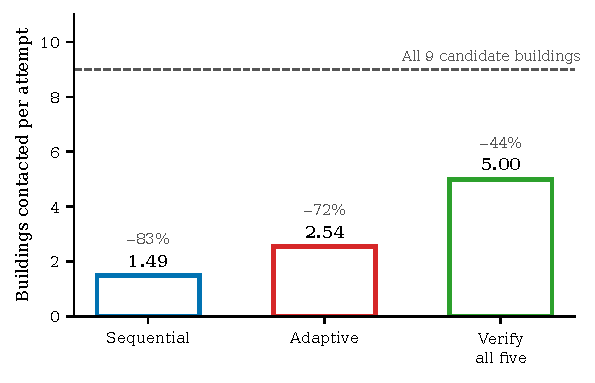
\includegraphics[width=0.62\textwidth]{figures/fig2_results.pdf}
\caption{Buildings contacted per identification attempt for routed visitors at 10 buildings (mean over 20 seeds). The dashed line marks the nine candidate buildings, which is the number contacted without routing; the percentages give the reduction relative to it.}
\label{fig:results}
\end{figure}

\begin{table}[!t]
\caption{Centralized search and the verification policies for routed visitors at 10 buildings and a shortlist of five: mean over 20 random seeds with 95\% confidence half-widths ($\pm$). The centralized baseline searches the 450 identities not registered in the capturing building and receives the captured embedding once. The adaptive policy uses a score-gap threshold of 5: all five shortlisted buildings are verified when the top two routing scores differ by at most 5, and the sequential rule is used otherwise. Payload is the captured-embedding traffic per attempt (2.048~KB per transmission).}\label{tab:adaptive}%
\begin{tabular}{@{}lcccc@{}}
\toprule
Method & Correct (\%) & Misidentified (\%) & Buildings & Payload (KB) \\
\midrule
Centralized (450 identities) & $95.50 \pm 0.25$ & $1.31 \pm 0.10$ & -- & 2.0 \\
Sequential & $92.19 \pm 0.28$ & $2.06 \pm 0.12$ & 1.49 & 3.1 \\
Adaptive & $92.95 \pm 0.28$ & $1.30 \pm 0.11$ & 2.54 & 5.2 \\
Verify all five & $92.81 \pm 0.29$ & $1.44 \pm 0.10$ & 5.00 & 10.2 \\
\bottomrule
\end{tabular}
\end{table}

\subsection{Bloom-Filter False-Positive Rate}
\label{sec:fpr}

The Bloom filters are configured for a false-positive probability of 1\%, whereas the effective rate, measured by testing the enrolled items of the other nine buildings against each filter, is $3.54 \pm 0.02\%$. Without a Bloom array, $2.61 \pm 0.02\%$ of the items of other buildings already equal an enrolled item in the same slot, close to the 2.41\% expected if the codes of 50 occupants were evenly distributed over $2^{11}=2048$ values, whereas the Bloom array alone yields $0.94 \pm 0.01\%$ on random integers that were never inserted. The excess over the configured target originates from collisions between LSH codes of different occupants and not from the Bloom array, so a positive filter response is a candidate signal and not evidence that an occupant is registered in the building.

\subsection{Communication Cost}
\label{sec:cost}

The costs are computed from message sizes and the measured number of buildings contacted, and they exclude protocol headers, replies, filter updates, computation time, and the caching of reference embeddings. A 512-dimensional float32 embedding occupies 2,048 bytes, so an attempt contacting $q$ buildings generates $2048q$ bytes. A central database of the 10,000 reference embeddings occupies 20.5~MB, whereas the distributed design shares ten Bloom filters of 7.3~KB each (73~KB in total), which every building holds, and each building retains 2.05~MB of reference embeddings locally. An attempt costs 3.1~KB under sequential verification (1.49 buildings), 5.2~KB under adaptive verification (2.54 buildings), and 10.2~KB when all five shortlisted buildings are contacted, compared with 18.4~KB for contacting all nine candidate buildings; a central database receives the embedding once (2.0~KB) but holds all reference embeddings in one place. Routing a visitor requires $(B-1)\cdot L(1+P)=4{,}392$ filter lookups, which grow linearly with the number of buildings.

% ============================================================
% DISCUSSION
% ============================================================

\section{Discussion}
\label{sec:discussion}

The results indicate a trade-off between identification accuracy and the number of buildings contacted. Restricting verification to a shortlist reduces the number of reference databases consulted, but the building holding the correct identity may be excluded from it; this accounts for the 2.69 percentage-point difference from centralized search, since the misidentification rate differs by only 0.13 points. Sequential verification has the lowest cost but accepts incorrect identities more often, whereas the adaptive policy verifies all candidates only when the top scores are close. It attained the accuracy of verifying all five buildings while contacting approximately half as many, although 37.6\% of attempts still required all five, so further reductions depend on a more discriminative ranking. The additional candidates caused by the 3.54\% false-positive rate are rejected by local verification, so the effect is on routing efficiency and not on the accepted identities. A further 3.3\% of visitors are accepted by an occupant of the capturing building before any routing takes place, an error that the routing stage cannot correct.

From a security perspective, the filters are derived from LSH codes of occupant embeddings, which preserve similarity. A party with access to the filters and the public hash parameters could test whether a given face produces filter hits for a building and infer that the person may be registered there, although no reference embedding is shared. This exposure was not measured here, and protecting the filters through access control, keyed hashing, or encryption is left for future work. Within the DSTS context, this study addresses the identification component and not the complete tracking and state-transition workflow.

% ============================================================
% CONCLUSION
% ============================================================

\section{Conclusion}
\label{sec:conclusion}

This work presented a routing strategy for decentralized face recognition across multiple buildings, in which per-building Bloom filters of LSH codes direct a captured face to the buildings that are likely to hold the matching reference, without a central database of reference embeddings. On 500 CASIA-WebFace identities distributed over 10 buildings, verifying all five shortlisted buildings achieved 92.81\% correct identification for routed visitors against 95.50\% for centralized search, and the adaptive policy achieved 92.95\% while contacting 2.54 of the nine candidate buildings and an estimated 5.2~KB of captured-embedding payload per attempt on average. The reduction in contacted buildings is accompanied by a loss of recall when the correct building is not shortlisted, and by a false-positive rate that LSH code collisions raise above the Bloom-filter design value. Future work includes evaluation on a larger and more varied population, more reliable candidate ranking, protection of the shared filters, identification of unknown visitors with a stricter acceptance rule, and measurement of communication costs in a deployed system.

% ============================================================
% LIMITATIONS
% ============================================================

\section{Limitations}
\label{sec:limitations}

The evaluation uses 500 identities from a single public dataset and 10 buildings, and the confidence intervals reflect variation in building assignment, hash randomness and the simulated day rather than a different population. The values $K=11$ and $P=3$ were chosen after observing accuracy on the test images, and the overlap between the ArcFace training data and CASIA-WebFace was not checked. The evaluation is closed-set, so the acceptance rule was not assessed for unknown individuals, including visitors enrolled nowhere, and the 3.3\% of visitors accepted by the capturing building are not recovered by routing. Communication costs are computed from message sizes, and latency, throughput, and filter synchronization were not measured. The encrypted channel and visitor caching were not implemented, no security analysis of the shared filters was carried out, and no formal privacy guarantee is established. A Bloom filter cannot delete items, so a change in enrollment requires rebuilding it.

\bmhead{Acknowledgement}

The authors gratefully acknowledge Sri Mata Amritanandamayi Devi (Amma), Chancellor, Amrita Vishwa Vidyapeetham, for her inspiration and for providing financial support for the Article Processing Charges (APC) of this publication.

\bibliography{akd}% akd.bib

\end{document}
